\documentclass[a4paper,12pt]{extarticle}
\usepackage[utf8x]{inputenc}
\usepackage[T1,T2A]{fontenc}
\usepackage[russian]{babel}
\usepackage{hyperref}
\usepackage{indentfirst}
\usepackage{listings}
\usepackage{color}
\usepackage{here}
\usepackage{array}
\usepackage{multirow}
\usepackage{graphicx}
\usepackage{amsmath}
\usepackage{amssymb}
\usepackage{makeidx}    

\usepackage{caption}
\renewcommand{\lstlistingname}{Программа} % заголовок листингов кода

\bibliographystyle{ugost2008ls}

\usepackage{listings}
\lstset{ %
extendedchars=\true,
keepspaces=true,
language=C,						% choose the language of the code
basicstyle=\footnotesize,		% the size of the fonts that are used for the code
numbers=left,					% where to put the line-numbers
numberstyle=\footnotesize,		% the size of the fonts that are used for the line-numbers
stepnumber=1,					% the step between two line-numbers. If it is 1 each line will be numbered
numbersep=5pt,					% how far the line-numbers are from the code
backgroundcolor=\color{white},	% choose the background color. You must add \usepackage{color}
showspaces=false				% show spaces adding particular underscores
showstringspaces=false,			% underline spaces within strings
showtabs=false,					% show tabs within strings adding particular underscores
frame=single,           		% adds a frame around the code
tabsize=2,						% sets default tabsize to 2 spaces
captionpos=t,					% sets the caption-position to top
breaklines=true,				% sets automatic line breaking
breakatwhitespace=false,		% sets if automatic breaks should only happen at whitespace
escapeinside={\%*}{*)},			% if you want to add a comment within your code
postbreak=\raisebox{0ex}[0ex][0ex]{\ensuremath{\color{red}\hookrightarrow\space}},
texcl=true,
inputpath=source,                     % директория с листингами
}

\usepackage[left=2cm,right=2cm,
top=2cm,bottom=2cm,bindingoffset=0cm]{geometry}

%% Нумерация картинок по секциям
\usepackage{chngcntr}
\counterwithin{figure}{section}
\counterwithin{table}{section}

%%Точки нумерации заголовков
\usepackage{titlesec}
\titlelabel{\thetitle.\quad}
\usepackage[dotinlabels]{titletoc}

%% Оформления подписи рисунка
\addto\captionsrussian{\renewcommand{\figurename}{Рисунок}}
\captionsetup[figure]{labelsep = period}

%% Подпись таблицы
\DeclareCaptionFormat{hfillstart}{\hfill#1#2#3\par}
\captionsetup[table]{format=hfillstart,labelsep=newline,justification=centering,skip=-10pt,textfont=bf}

%% Путь к каталогу с рисунками
\graphicspath{{pictures/}}


\begin{document}	% начало документа

% Титульная страница
\begin{titlepage}	% начало титульной страницы

	\begin{center}		% выравнивание по центру

		\large Санкт-Петербургский Политехнический Университет Петра Великого\\
		\large Институт компьютерных наук и технологий \\
		\large Кафедра компьютерных систем и программных технологий\\[6cm]
		% название института, затем отступ 6см
		
		\huge Телекоммуникационные технологии\\[0.5cm] % название работы, затем отступ 				%0,5см
		\large Отчет по лабораторной работе №3\\[0.1cm]
		\large Линейная фильтрация
		\\[5cm]

	\end{center}


	\begin{flushright} % выравнивание по правому краю
		\begin{minipage}{0.25\textwidth} % врезка в половину ширины текста
			\begin{flushleft} % выровнять её содержимое по левому краю

				\large\textbf{Работу выполнил:}\\
				\large Балсутьев В.А.\\
				\large {Группа:} 33501/4\\
				
				\large \textbf{Преподаватель:}\\
				\large Богач Н.В.

			\end{flushleft}
		\end{minipage}
	\end{flushright}
	
	\vfill % заполнить всё доступное ниже пространство

	\begin{center}
	\large Санкт-Петербург\\
	\large \the\year % вывести дату
	\end{center} % закончить выравнивание по центру

\thispagestyle{empty} % не нумеровать страницу
\end{titlepage} % конец титульной страницы

\vfill % заполнить всё доступное ниже пространство
	

% Содержание
% Содержание
\renewcommand\contentsname{\centerline{Содержание}}
\tableofcontents
\newpage




\section{Цель работы}
Познакомиться со средствами генерации и визуализации простых сигналов, c различными программными средствами цифоровой обработки сигнала, научиться ими пользоваться вследствие выполнения поставленных задач.


\section{Постановка задачи}
В командном окне MATLAB и в среде Simulink промоделировать сигналы из Главы 3, сс. 150–170 (см. Справочные материалы). В качестве альтернативного программного средства можно использовать язык python и различные сопутствующие инструменты(Jupyter Notebook). После выполнения моделирования так же требуется оформить отчет с помощью LaTeX

\section{Теоретическая информация}
В качестве языка выбираем python 3. Основные библиотеки, которые нам потребуются:

\begin{itemize}
\item scipy.signal - для обработки сигналов
\item matplotlib - для построения графиков
\item numpy - для удобной работы с матрицами и векторами
\end{itemize}


Для моделирования и выполнения кода будем использовать Jupyter Notebook.
Приведем некоторые формулы, которые будут использоваться в данной работе:

\begin{itemize}

\item гармонический сигнал:
	 \begin{equation}\label{eq1} 	
	 	s_1(t) = \cos(2\pi f_0t +\phi)  
	 \end{equation}
\item затухающий гармонический сигнал:
    \begin{equation}\label{eq2} 
    	s_2(t) = \cos(2\pi f_0t+\phi)e^{-\alpha t}
    \end{equation}
\item Гауссов импульс:
    \begin{equation}\label{eq3} 
    	y(t) = \cos(2\pi f_ct)e^{-\alpha t^2} 
    \end{equation}
\item Функция Дирихле:
	\begin{equation}\label{eq4}  
		\dfrac{\sin(nx/2)}{nsin(nx/2)}, n \in \mathbb Z 			
	\end{equation}
			
\end{itemize}

\section{Ход работы}
Для реализации гармонического сигнала в соответствии с формулой (\ref{eq1})
нам необходимо также реализовать функцию поэлементного умножения elem\_multiple по аналогии с MATLAB. 

\subsection{Введение}

\lstinputlisting[
	label=code:source01,
	caption={source01.py},% для печати символ '_' требует выходной символ '\'
]{source/source01.py}
\parindent=1cm % командна \lstinputlisting сбивает параментры отступа
Выполнив данный код, получаем график сигнала:
\begin{figure}[H]
	\begin{center}
		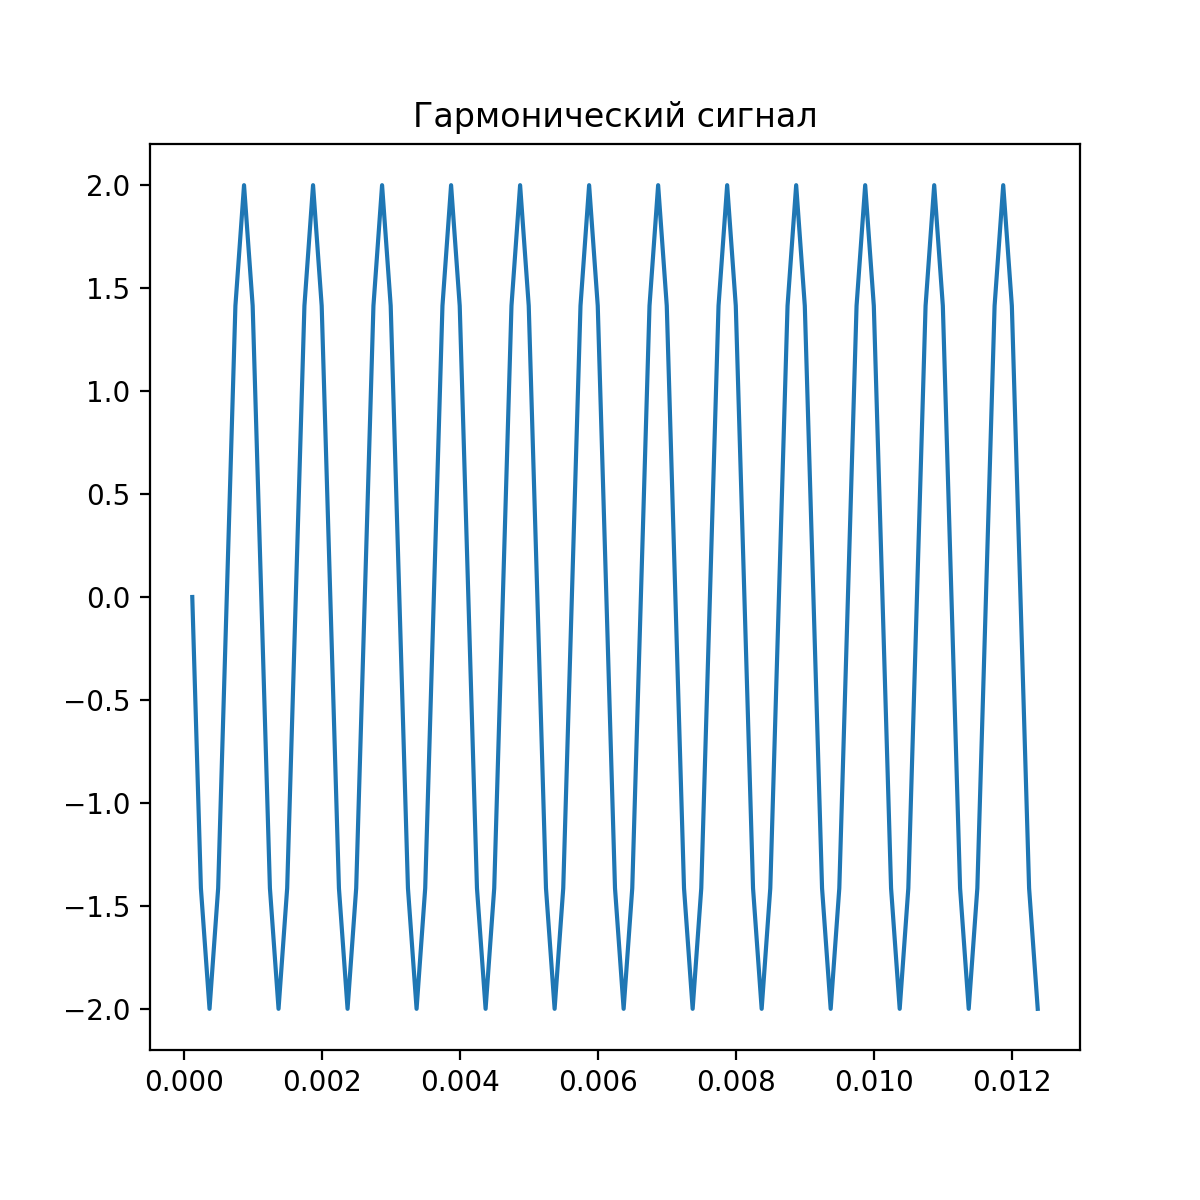
\includegraphics[scale=0.7]{001harmonic.png}
		\caption{Гармонический сигнал} 
		\label{pic:pic01} % название для ссылок внутри кода
	\end{center}
\end{figure}


\noindent Далее реализуем уже затухающий гармонический сигнал (\ref{eq2}):

\lstinputlisting[
	label=code:source02,
	caption={source02.py},% для печати символ '_' требует выходной символ '\'
]{source/source02.py}
\parindent=1cm % командна \lstinputlisting сбивает параментры отступа
\noindent  Выполнив данный код, получаем график сигнала:
\begin{figure}[H]
	\begin{center}
		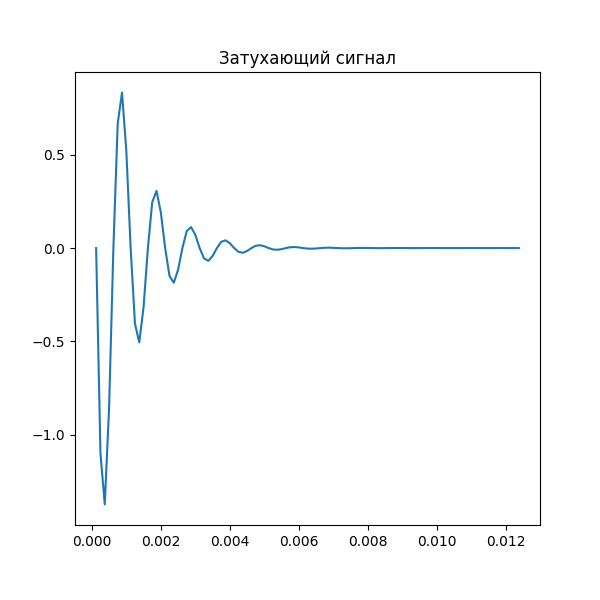
\includegraphics[scale=0.7]{002harmonic.png}
		\caption{Затухающий гармонический сигнал} 
		\label{pic:pic02} % название для ссылок внутри кода
	\end{center}
\end{figure}

Далее промоделируем многоканальный сигнал (у каждого канала будет просто своя частота), взяв число канальности равное 5. Сигнал будет так же гармоническим: \\
$s_3(t) = \cos(2\pi f_0t)$, где $f_0= (600, 800, 1000, 1200, 1400)$ 

\lstinputlisting[
	label=code:source03,
	caption={source03.py},% для печати символ '_' требует выходной символ '\'
]{source/source03.py}
\parindent=1cm % командна \lstinputlisting сбивает параментры отступа
\noindent  Выполнив данный код, получаем график сигнала:
\begin{figure}[H]
	\begin{center}
		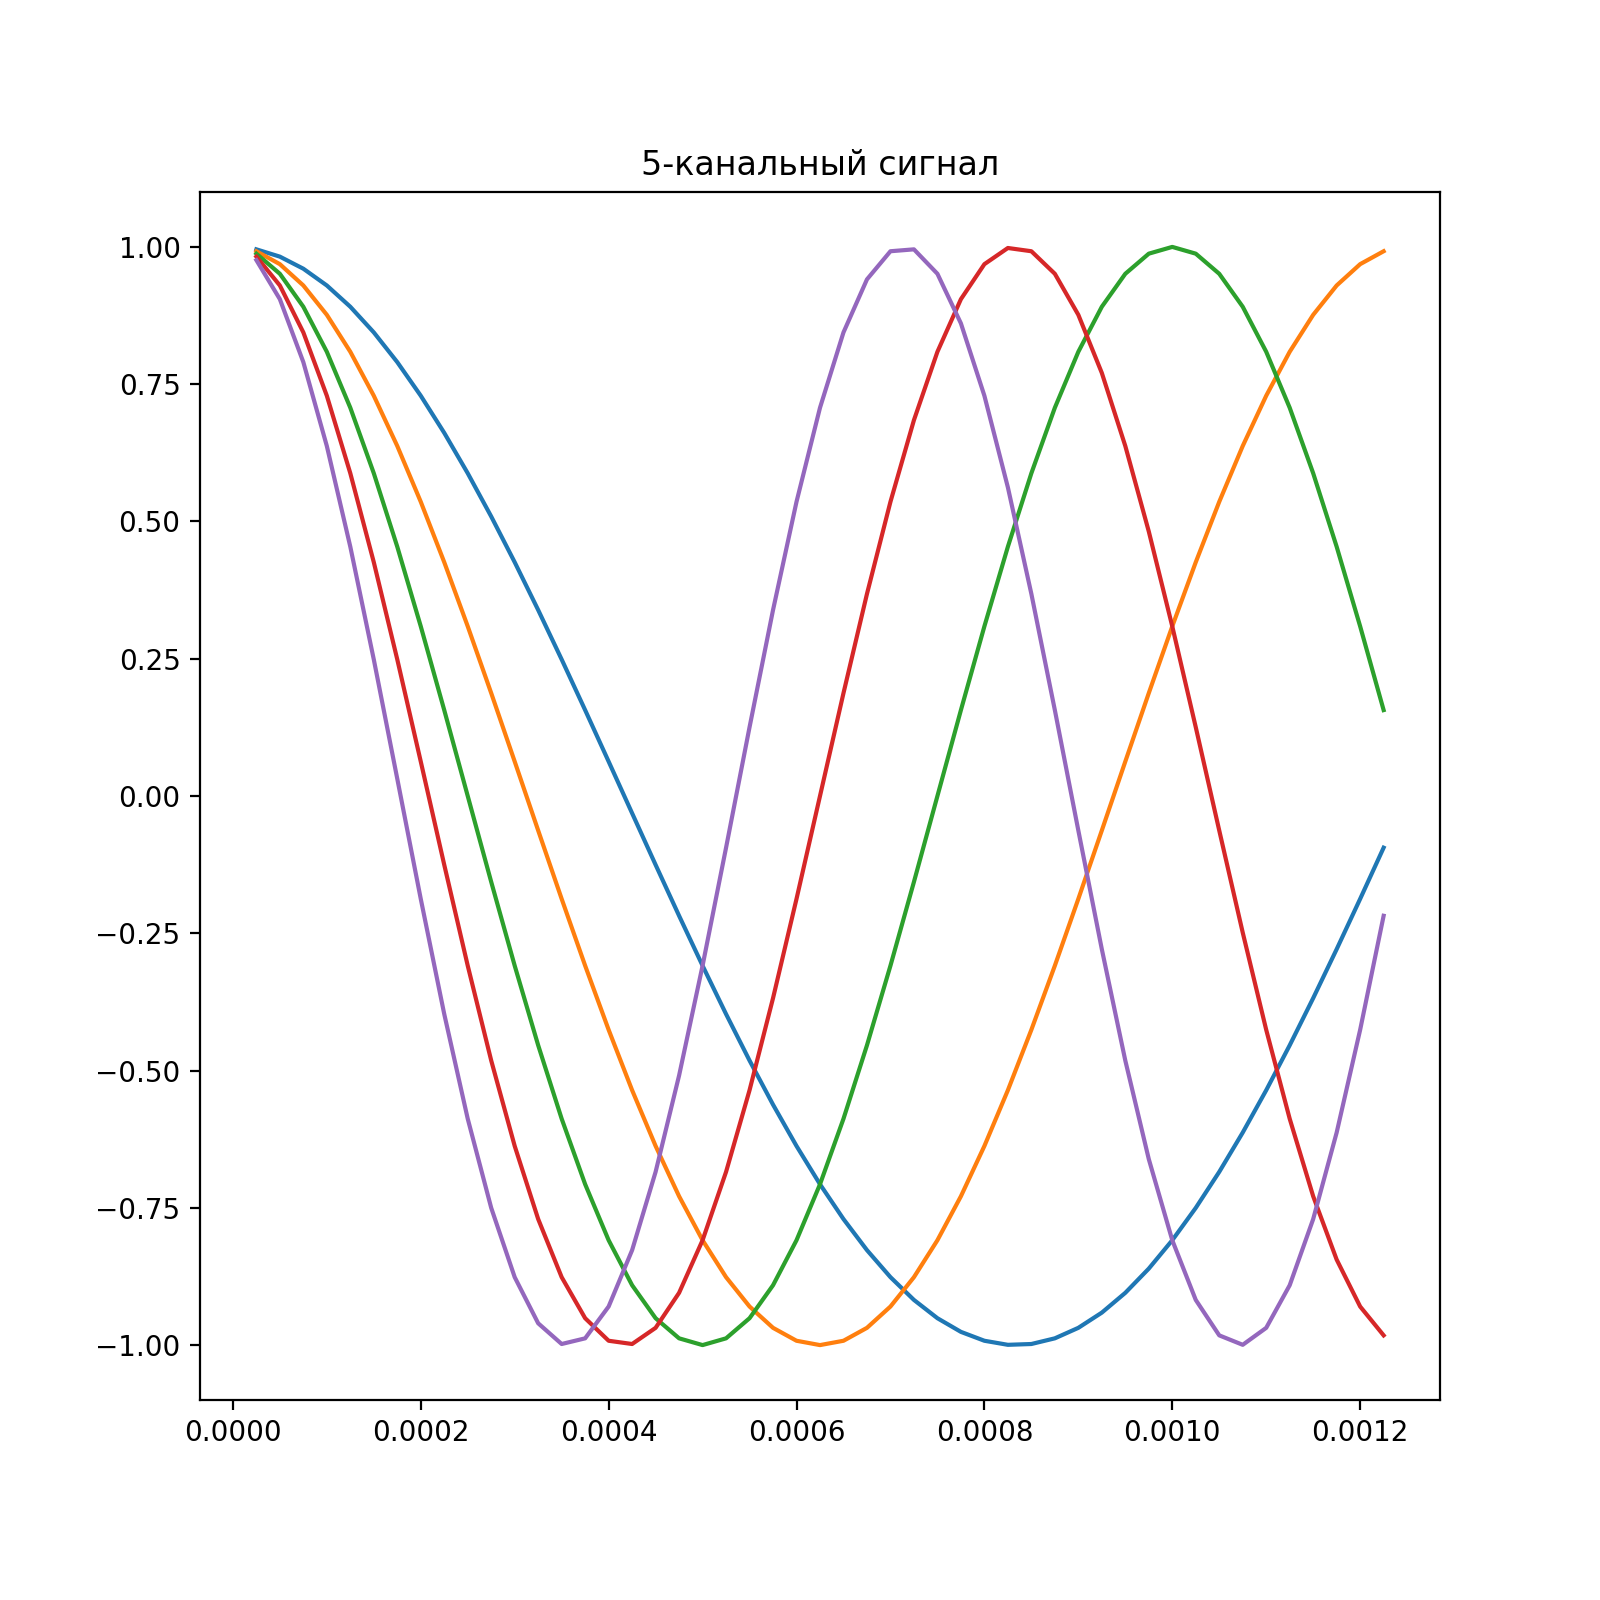
\includegraphics[scale=0.7]{/003_5chnls.png}
		\caption{Многоканальный сигнал} 
		\label{pic:pic03} % название для ссылок внутри кода
	\end{center}
\end{figure}
В соотвествии с теорией получаем семейство косинусов с различными фазами - искомый многоканальный сигнал.

\subsection{Одиночные импульсы}

В библиотеке python scipy.signal в отличие от MATLAB нет функций генерации одиночных имплусов, поэтому для примера реализуем прямоуголный импульс самостоятельно.  
\lstinputlisting[
	label=code:source04,
	caption={source04.py},% для печати символ '_' требует выходной символ '\'
]{source/source04.py}
\parindent=1cm % командна \lstinputlisting сбивает параментры отступа
\noindent  Выполнив данный код, получаем график сигнала:
\begin{figure}[H]
	\begin{center}
		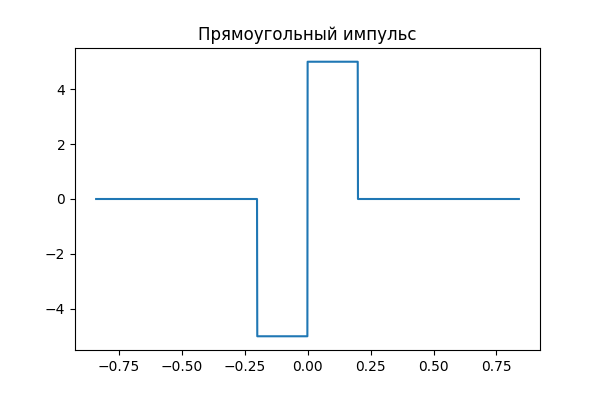
\includegraphics[scale=0.7]{004rectImp.png}
		\caption{Прямоугольный импульс} 
		\label{pic:pic04} % название для ссылок внутри кода
	\end{center}
\end{figure}
Полученный график очевидно является прямоугольным импульсом. 

Также построим импульс Гаусса, реализация которого представлена в scipy.signal. По определению Гауссов импульс представляется формулой (\ref{eq3}).

\lstinputlisting[
	label=code:source05,
	caption={source05.py},% для печати символ '_' требует выходной символ '\'
]{source/source05.py}
\parindent=1cm % командна \lstinputlisting сбивает параментры отступа
\noindent  Выполнив данный код, получаем график сигнала:
\begin{figure}[H]
	\begin{center}
		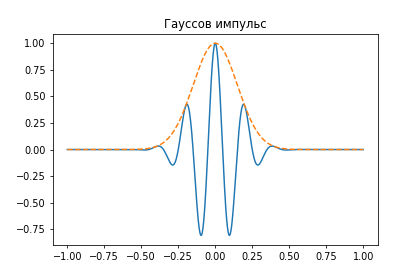
\includegraphics[scale=0.7]{005_gaus.png}
		\caption{Импульс Гаусса} 
		\label{pic:pic05} % название для ссылок внутри кода
	\end{center}
\end{figure}

Кроме сигнала, для примера так же построили и спектр Гауссова импульса.
\begin{figure}[H]
	\begin{center}
		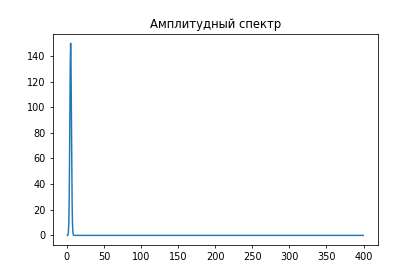
\includegraphics[scale=0.7]{006_spctrgaus.png}
		\caption{Спектр Импульс Гаусса} 
		\label{pic:pic06} % название для ссылок внутри кода
	\end{center}
\end{figure}

\subsection{Генерация периодических сигналов}
Периодические сигналы - это функции, которые позволяют формировать отсчеты периодических сигналов различной формы. Рассмотрим последовательность уже знакомых прямоугольных импульсов.

\lstinputlisting[
	label=code:source06,
	caption={source06.py},% для печати символ '_' требует выходной символ '\'
]{source/source06.py}
\parindent=1cm % командна \lstinputlisting сбивает параментры отступа
\noindent  Выполнив данный код, получаем график сигнала:
\begin{figure}[H]
	\begin{center}
		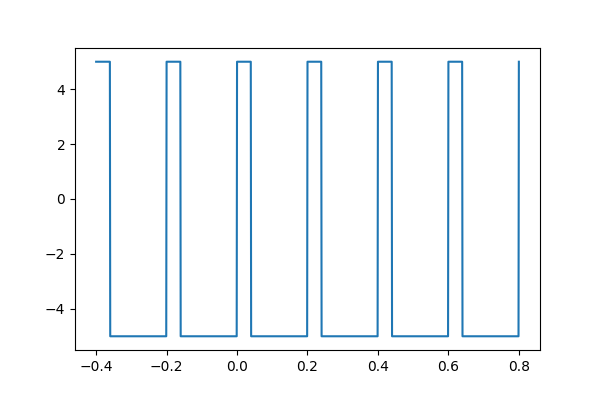
\includegraphics[scale=0.7]{007rectImplses.png}
		\caption{Прямоугольный периодический сигнал} 
		\label{pic:pic07} % название для ссылок внутри кода
	\end{center}
\end{figure}

C помощью функции sawtooth из scipy.signal реализуем последовательность треугольных импульсов.

\lstinputlisting[
	label=code:source07,
	caption={source07.py},% для печати символ '_' требует выходной символ '\'
]{source/source07.py}
\parindent=1cm % командна \lstinputlisting сбивает параментры отступа
\noindent  Выполнив данный код, получаем график сигнала:
\begin{figure}[H]
	\begin{center}
		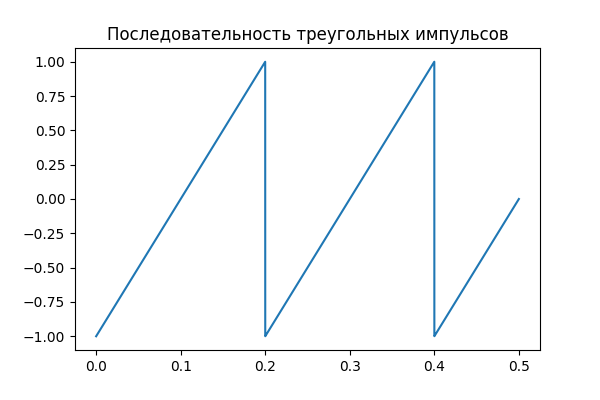
\includegraphics[scale=0.7]{008_sawtooth.png}
		\caption{Последовательность треугольных импульсов} 
		\label{pic:pic08} % название для ссылок внутри кода
	\end{center}
\end{figure}

Реализуем также функцию Дирихле(\ref{eq4}):

\lstinputlisting[
	label=code:source09,
	caption={source08.py},% для печати символ '_' требует выходной символ '\'
]{source/source08.py}
\parindent=1cm % командна \lstinputlisting сбивает параментры отступа
\noindent  Выполнив данный код, получаем график сигнала:
\begin{figure}[H]
	\begin{center}
		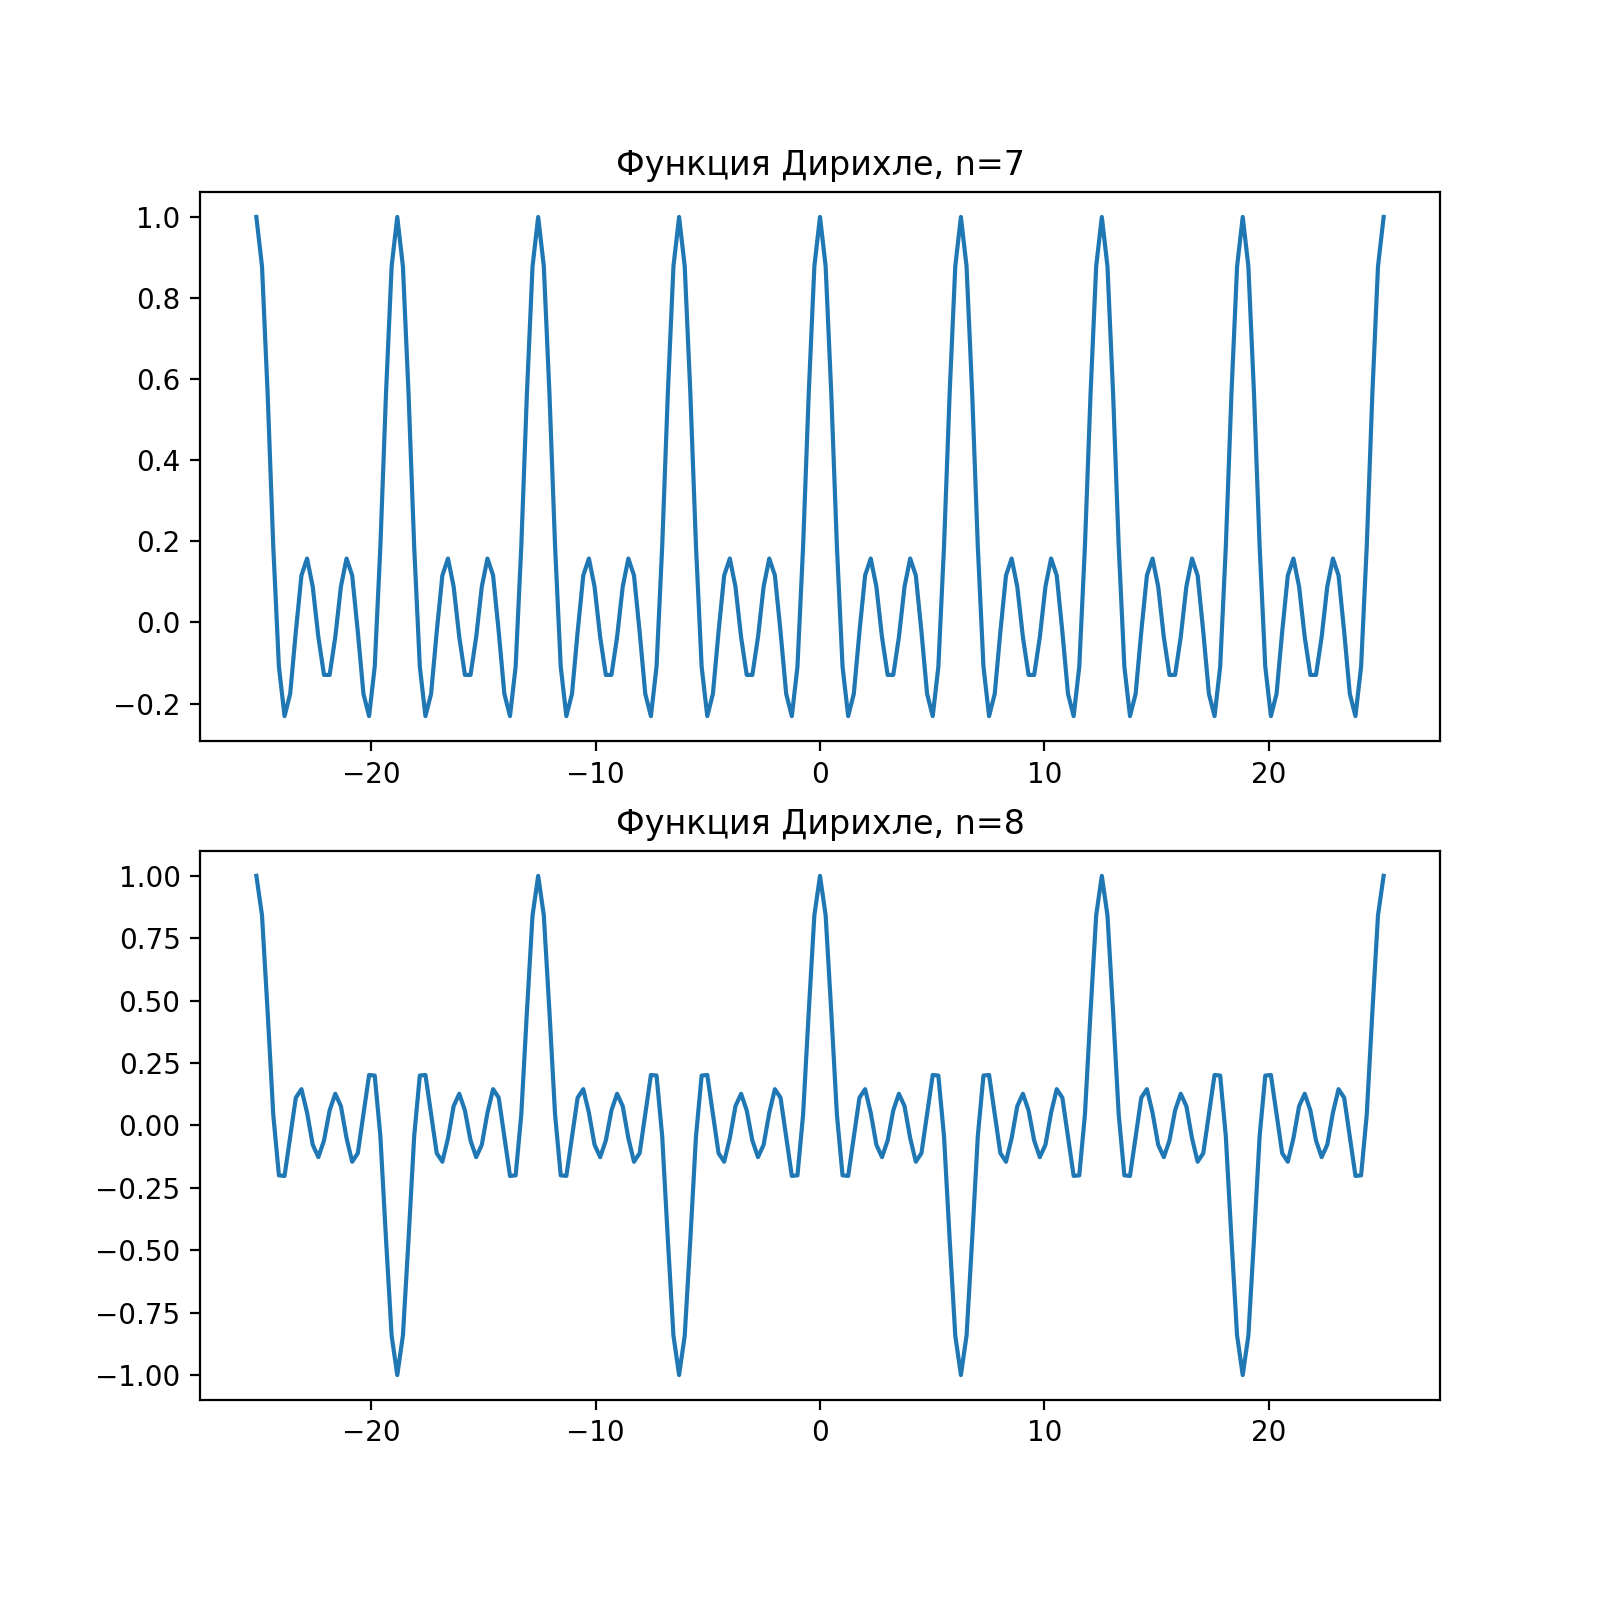
\includegraphics[scale=0.7]{009_dirichle.png}
		\caption{Функции Дирихле 7 и 8 степеней} 
		\label{pic:pic09} % название для ссылок внутри кода
	\end{center}
\end{figure}


%\subsection{Частичный листинг}
% настрока частичного ввода (требуется один раз)
%\makeatletter
%\def\lst@PlaceNumber{\llap{\normalfont
%                \lst@numberstyle{\the\lst@lineno}\kern\lst@numbersep}}
%\makeatother

%\lstinputlisting[
%	label=code:hello_mod,
%	linerange={4-5},
%	caption={фрагмент hell\_o.c},
%]{hell_o.c}
%\parindent=1cm

%\subsection{Таблица}

%\begin{table}[H]
%	\caption{ Название таблицы}
%	\begin{center}
%		\begin{tabular}{|l|l|}
%			\hline
%			top left & top right\\ \hline
%			bot left & bot right\\ \hline
%		\end{tabular}
%		\label{tabular:tab_examp}
%	\end{center}
%\end{table}

\section{Вывод}

В результате выполнению данной работы нам удалось получить элементарные навыки использования python и JupyterNotebook для анализа и моделирования сигналов.
Также мы узнали о различных видах сигналов:

\begin{itemize}
	\item[-]  гармонические сигналы 
	\item[-] одиночные импульсы
	\item[-] периодические сигналы
	\item[-] сигналы с меняющейся частотой
\end{itemize}

\end{document}
